\documentclass{article}
\usepackage{tikz}
\begin{document}
% 形状变换
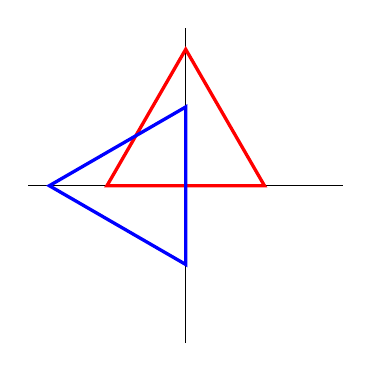
\begin{tikzpicture}
    % rotate - 旋转, 旋转点为(0,0)
    \draw (-2,0) -- (2,0);
    \draw (0,-2) -- (0,2);
    \draw[red, very thick] (-1,0)++(60:2) -- (-1,0) -- (1,0) -- cycle;
    \draw[rotate=90, blue, very thick] (-1,0)++(60:2) -- (-1,0) -- (1,0) -- cycle;
\end{tikzpicture}\\\vspace{2cm}

\begin{tikzpicture}
    % shift - 偏移
    \draw (0,0) -- (2,0);
    \draw[purple, shift={(-1,-1)}] (0,0) -- (2,0);
\end{tikzpicture}\\\vspace{2cm}

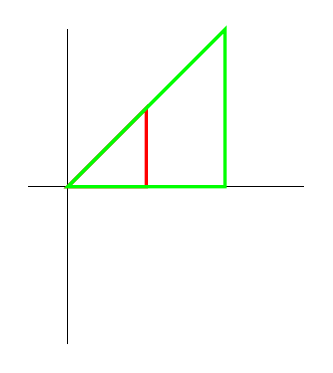
\begin{tikzpicture}
    % scale - 伸缩
    \draw (-0.5,0) -- (3,0);
    \draw (0,-2) -- (0,2);
    \draw[red, very thick] (0,0) -- (1,1) -- (1,0) --cycle;
    \draw[scale=2, green, very thick] (0,0) -- (1,1) -- (1,0) --cycle;
\end{tikzpicture}\\\vspace{2cm}

\begin{tikzpicture}
    % slant - 倾斜
    \draw (-3.5,0) -- (3.5,0);
    \draw (0,-3.5) -- (0,3.5);
    \draw (0,0) -- (1,1) -- (1,0);
    \draw[xslant=2,red,opacity=0.5] (0,0) -- (1,1) -- (1,0);
    \draw[yslant=2,blue,opacity=0.5] (0,0) -- (1,1) -- (1,0);
\end{tikzpicture}
\end{document}
